\documentclass[12pt]{paper}
\bibliographystyle{IEEEtran}
\usepackage{chapterbib,parskip,color,glossaries,makeidx,graphicx}
\setlength{\parskip}{.5cm plus4mm minus3mm}
\renewcommand*{\refname}{}
%\renewcommand{\bibsection}{\subsection{References}}

\usepackage[margin=1in]{geometry}
\usepackage[colorlinks, pdfborder={0 0 0}, hypertex]{hyperref}
\definecolor{darkblue}{rgb}{0,0,0.5}
\hypersetup{
    colorlinks=true,
    urlcolor=blue,
    citecolor=black,
    linkcolor=darkblue
}
\renewcommand{\glossarysection}[2][]{}
\makeglossaries
\makeindex
%\makeatletter
%  \renewcommand\@seccntformat[1]{\csname the#1\endcsname.\quad}
%\makeatother
%\def\thesection {\Alph{section}}
%\def\thesubsection {\alph{subsection}}
%\def\thesubsubsection {\arabic{subsubsection}}
%\usepackage{titlesec}
%\titlespacing{\subsection}{2em}{0pt}{0pt}
\hyphenation{op-tical net-works semi-conduc-tor}
%\usepackage{longtable}

\title{Software Requirements Specification v2.0} 

\author{\hfill \hspace{4.09in} Ryan Alcoran\\ \hfill Joe Lee\\ \hfill
  Shivalik Narad\\ \hfill Nam Phan\\ \hfill Swapna Vemparala\\ \hfill
  Amber Wong\\[2em] \hfill {\bf CS 160 SQ06}}

\makeglossaries
\newglossaryentry{cloud}{ 
  name=cloud,
  description={servers hosted online that are used to store, manage, 
    and access data}
}
\newglossaryentry{database}{
  name=database,
  description={collection of all information that will be used by the
    SiQuoia system}
}
\newglossaryentry{gamer}{
  name=gamer,
  description={see {\it user}}
}
\newglossaryentry{MCQ}{
  name=MCQ,
  description={multiple choice quiz}
}
\newglossaryentry{product}{
  name=product,
  description={the multiple choice quiz game known as SiQuoia}
}
\newglossaryentry{progress analysis}{
  name={progress analysis},
  description={the user's highest quiz score (most number of questions
    answered correctly) in a particular quiz packet, as well as the
    combined score percentage of all quizzes}
}
\newglossaryentry{SeQuoia}{
  name=SeQuoia,
  description={the company SiQuoia, Inc}
}
\newglossaryentry{SiQuoia}{
  name=SiQuoia,
  description={Simple Intelligence Quotient Increasing Application}
}
\newglossaryentry{SqQuoia}{
  name=SqQuoia,
  description={next generation common platform for running and
    managing quiz games that carter to increasing intelligence
    quotient and provides training and certification processes}
}
\newglossaryentry{user}{
  name=user,
  description={person(s) who operate or interact directly with the
    product}
}

\begin{document}
\begin{titlepage}
\maketitle

\begin{table}[b]
\centering
\begin{tabular}{|l|r|l|r|}
  \multicolumn{4}{l}{\bf Revision History} \\
  \hline
  Name                    & Date       & Reasons for changes  & Version \\
  \hline
  High-level requirements & 9/11/2013  & Initial creation     & 1 \\
  \hline
  Detailed requirements   & 9/29/2013  & Final draft          & 2 \\
  \hline
\end{tabular}
\end{table}

\end{titlepage}

\newpage
\tableofcontents

\section{Introduction}
\label{sec:introduction}

\subsection{Purpose}
\label{subsec:purpose}
The purpose of this document, which follows the structure outlined in
IEEE Std 830-1998~\cite{IEEE:830-1998}, is to provide a detailed
description of the quiz program known as \gls{SiQuoia}. It will
provide detailed descriptions of what this application will do,
including functions and features of the program, interfaces, and
constraints under which the program will operate. This document is
intended for stakeholders at SiQuoia, Inc., known hereafter as
\gls{SeQuoia}.

\subsection{Scope}
\label{subsec:scope}
The software system known as SiQuoia includes a simple quiz program
with packages consisting of one question and four answers, with only
one answer being correct. The program is designed to increase the
intelligence quotients of users or provide training or help in
certification processes. Each question will have a rank based on the
number of times it is answered correctly.

The system will have a web browser interface in which \glspl{user}
play as a guest or registered user. If registered, the system will
allow users to log in, resume their most recently unfinished quiz (if
such a quiz exists), select a game mode and begin a new quiz, view and
publish their progress analysis, and submit new quiz questions. The
system will also allow registered users to claim rewards in the game
store using cash or SiQuoia points and refer new users.

The web interface will interact with a database to keep track of user
and game information.

\subsection{Definitions, Acronyms, and Abbreviations}
\label{subsec:gls}
\printglossaries

\subsection{References}~\\[-9em]
\label{subsec:refs}
\bibliography{srs}

\subsection{Overview}
\label{subsec:overview}
The next section, Overall Description, will contain an overview of the
functions and features of the program. Following it, the third
section, Specific Requirements, will go further into detail about the
functions defined in section two.

\section{Overall Description}
\label{sec:overall}
\subsection{Product Perspective}
\label{subsec:perspective}
The SiQuoia program is independent of any other \gls{MCQ} gaming
systems and is intended to run separately from such systems. It relies
on a device with a browser and Internet access.

\begin{figure}[h!]
\centering
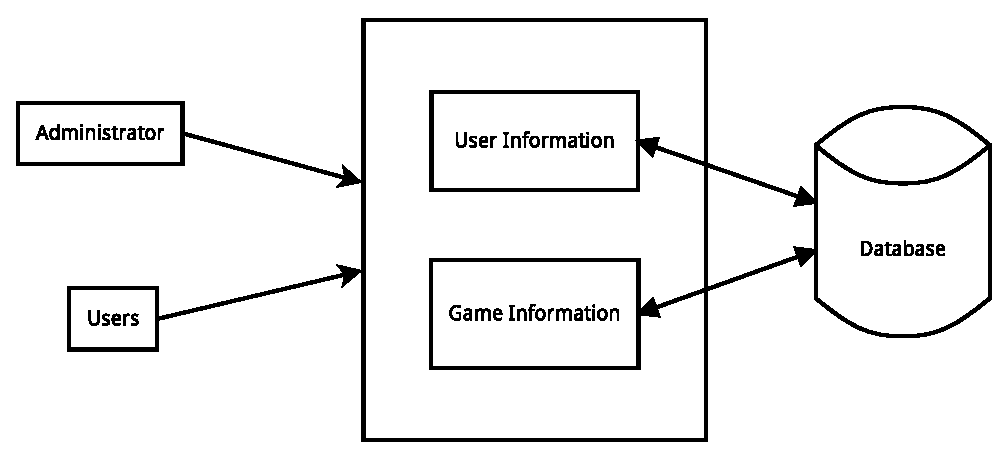
\includegraphics[width=\textwidth]{system-overview}
\caption{SiQuoia System Overview}
\end{figure}

The SiQuoia program will allow users and administrators to log in and
access the Web interface.  The interface interacts with the database
to display user information and game information.

\subsubsection{System Interfaces}
Refer to section~\ref{subsec:functions}

\subsubsection{User Interfaces}
SiQuoia will have one question per page and each question will have a
time limit of 20 seconds. The user will then be able to navigate to
the next question by clicking on the next button. At the end of the
quiz the user shall click on the finish button in order to the submit
the quiz for evaluation. SiQuoia will then provide the score to the
user soon after the test.

\subsubsection{Hardware Interfaces}
SiQuoia requires a keyboard and a mouse or touchpad.

\subsubsection{Software Interfaces}
None.

\subsubsection{Communication Interfaces}
The Server and Database components may be located on the same host.

\subsubsection{Memory}
SiQuoia shall require no more than 1~GB of RAM and 250~MB of secondary
storage.

\subsubsection{Operations}
SiQuoia shall operate in different modes such as Tutorial,Test and
Practice mode.This would depend on the user type i.e.) if the user is
a registered or a guest user.

SiQuoia shall save the state of the quiz so that it can be resumed
from the point it was paused, the timer shall also pause during this
time.

\subsubsection{Site Adaptation Requirements}
No specific site adaptation should be required.

\subsection{Product Functions}

\begin{figure}[h!]
\centering
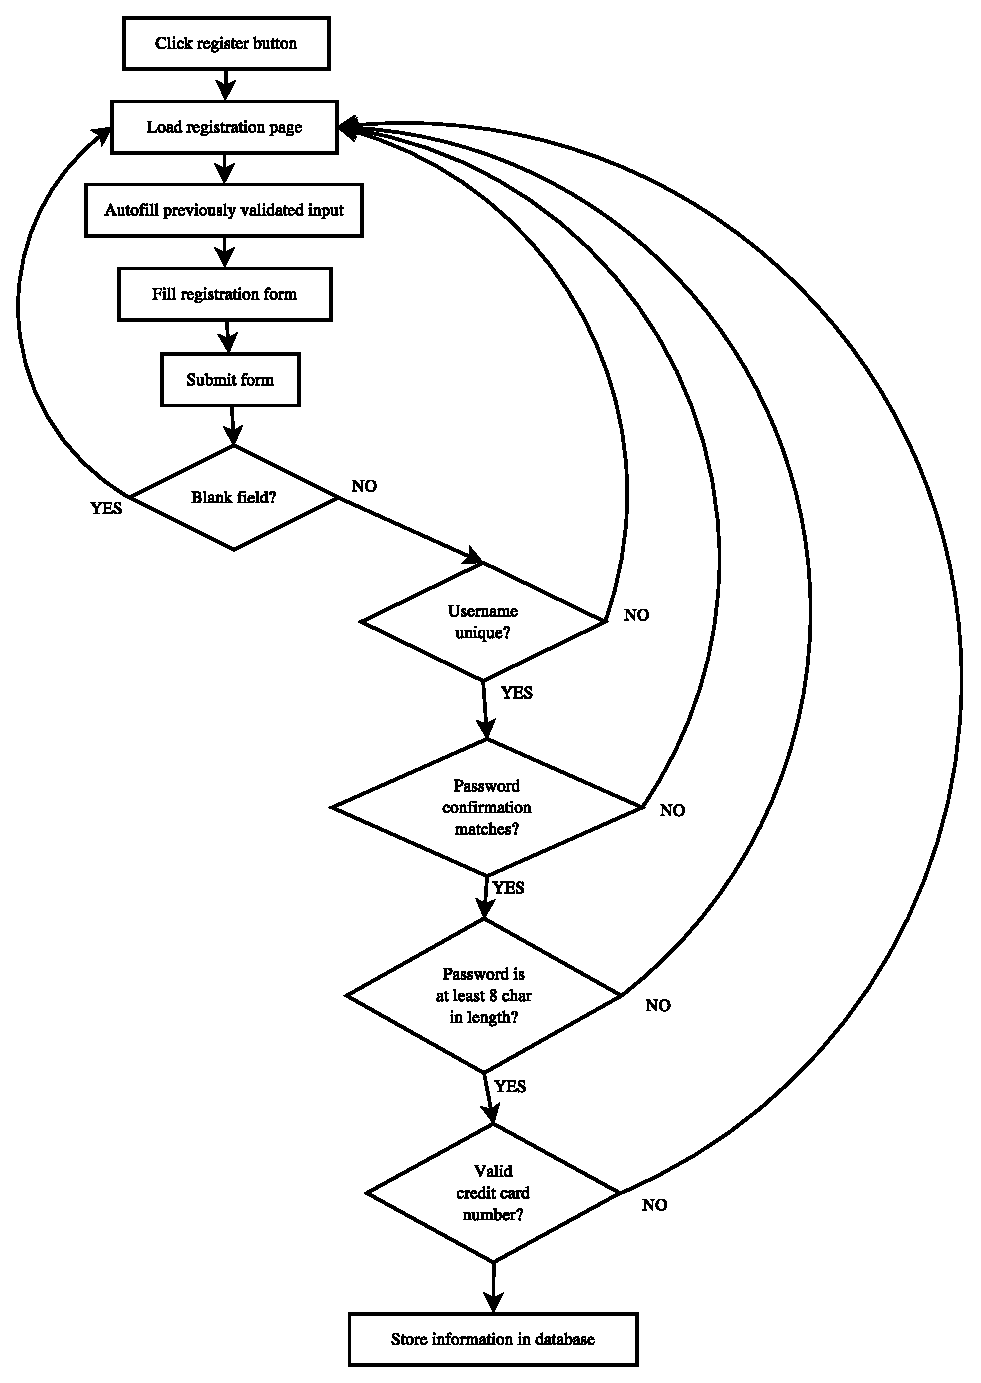
\includegraphics[width=0.9\textwidth]{flowcharts/registration}
\caption{Flow chart for user registration.}
\end{figure}

\begin{figure}[h!]
\centering
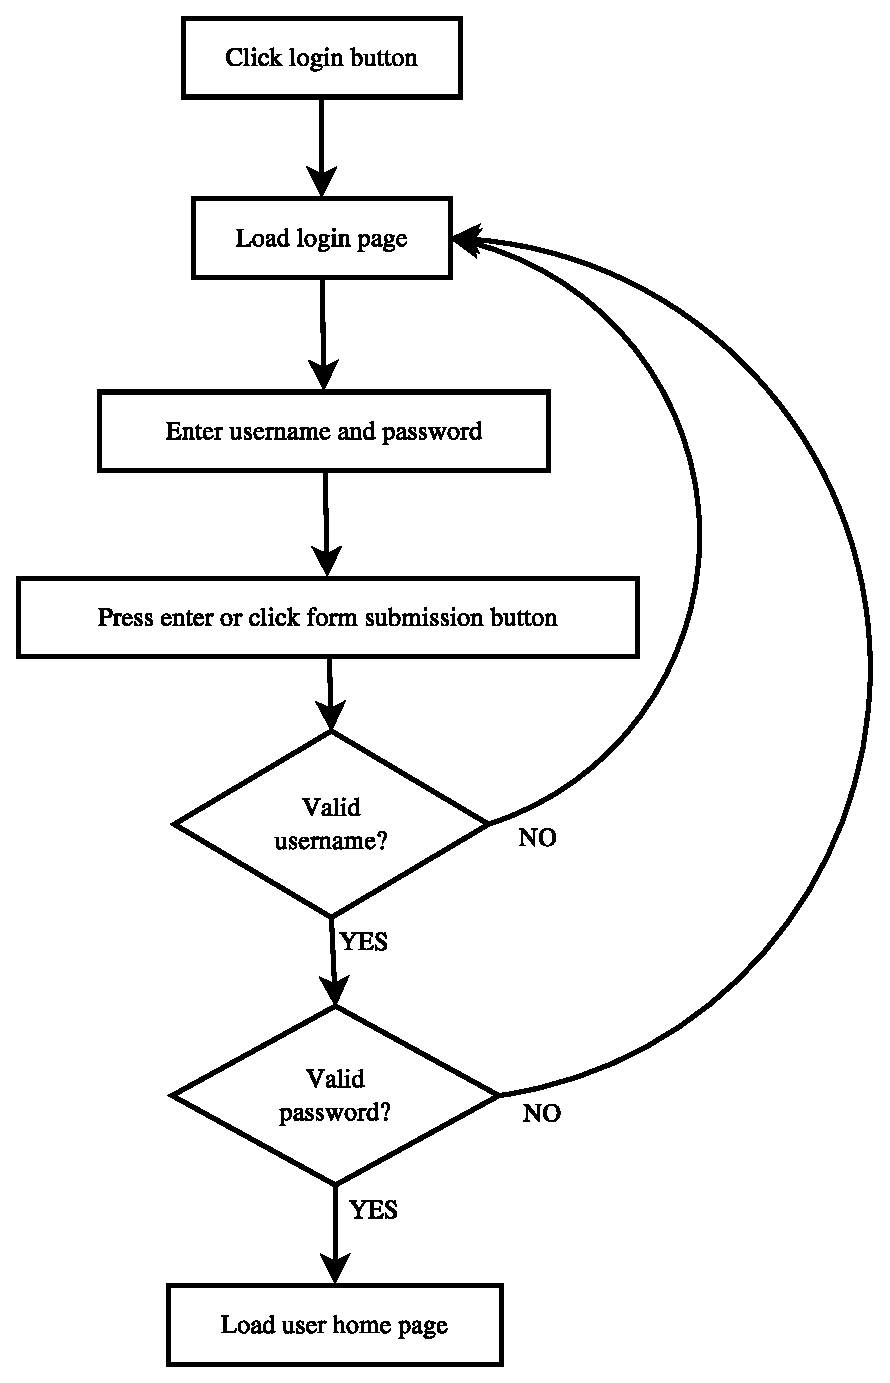
\includegraphics[width=0.7\textwidth]{flowcharts/login}
\caption{Flow chart for user registration.}
\end{figure}

\end{document}
